\subsubsection{Interleave}
Pour essayer de diminuer les effets NUMA, nous activons la politique d'allocation mémoire interleave.
%
Les pages mémoires sont donc distribuées uniformément entre chaque bancs NUMA.
%
Sur Rostand, la factorisation donne de bons résultats qu'avec une politique d'allocation first touch (Fig.~\ref{fig:res_facto_inter_rostand})
%
Par contre, nous obtenons une amélioration entre 3~\% et 30~\% de la résolution triangulaire (Fig.~\ref{fig:res_trsv_inter_rostand}).

%   (-_-)   %
\begin{figure}[t!]
  \centering
  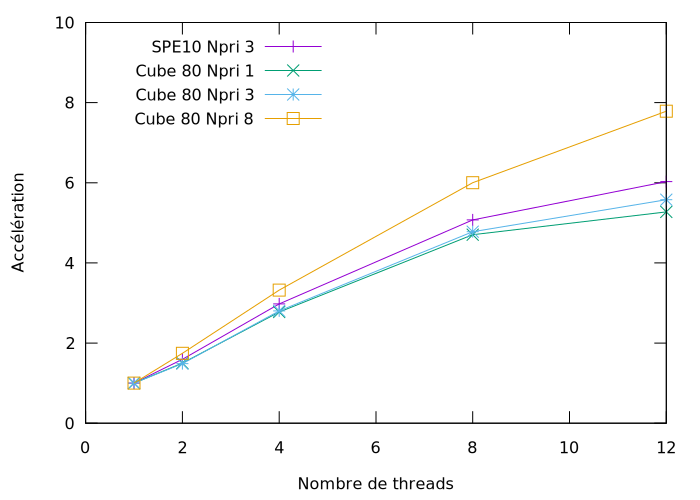
\includegraphics[width=0.7\textwidth]{res_facto_interleave}
  \caption{Performance de la factorisation sur Rostand avec une politique d'allocation interleave.}
  \label{fig:res_facto_inter_rostand}
\end{figure}


%   (-_-)   %
\begin{figure}[t!]
  \centering
  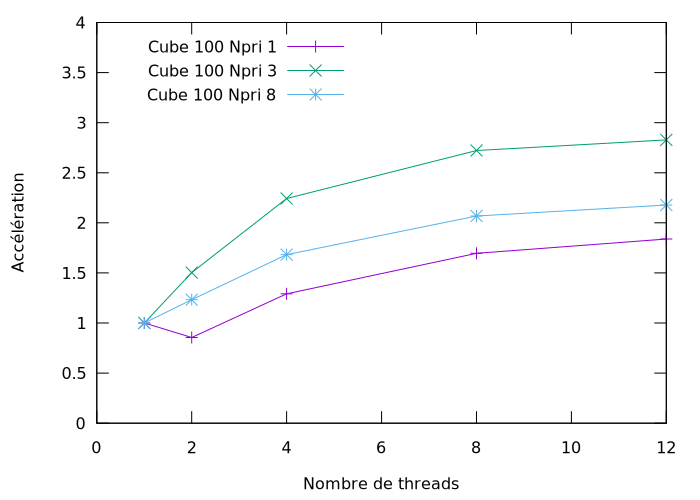
\includegraphics[width=0.7\textwidth]{res_trsv_interleave}
  \caption{Performance de la résolution triangulaire sur Rostand avec une politique d'allocation interleave.}
  \label{fig:res_trsv_inter_rostand}
\end{figure}

Sur Manumanu, la factorisation se comporte de la même façon que sur Rostand (Fig.~\ref{fig:res_facto_inter_manumanu}).
%
De même, l'accélération maximale de la résolution triangulaire est meilleure avec une politique d'allocation interleave (Fig.~\ref{fig:res_trsv_inter_manumanu}).


%   (-_-)   %
\begin{figure}[t!]
  \centering
  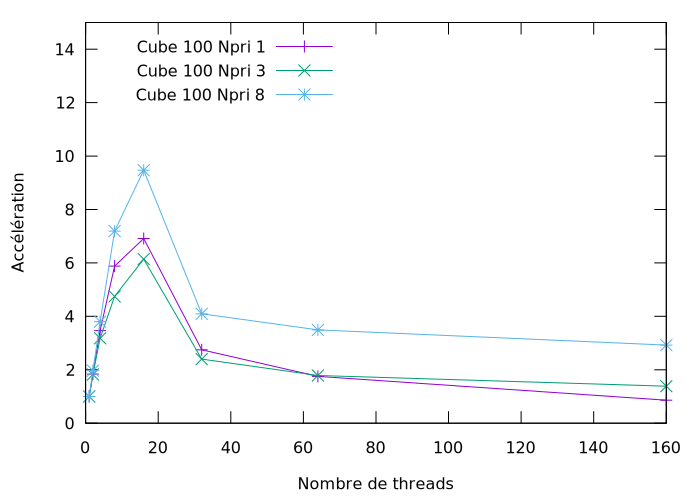
\includegraphics[width=0.7\textwidth]{res_facto_inter_manu}
  \caption{Performance de la factorisation sur Manumanu avec une politique d'allocation interleave.}
  \label{fig:res_facto_inter_manumanu}
\end{figure}


%   (-_-)   %
\begin{figure}[t!]
  \centering
  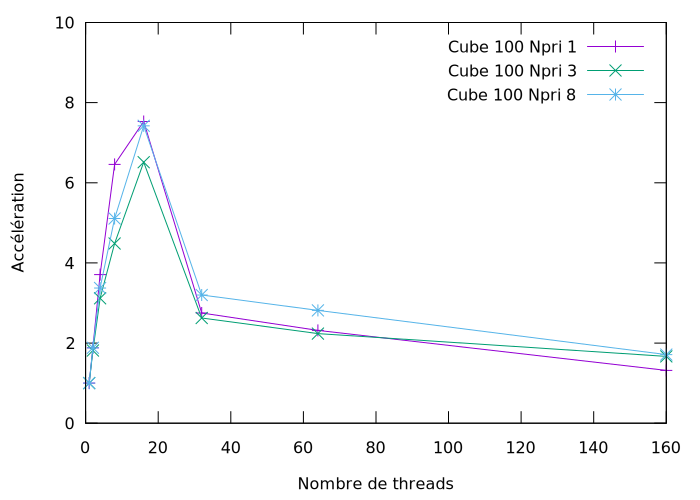
\includegraphics[width=0.7\textwidth]{res_trsv_inter_manu}
  \caption{Performance de la résolution triangulaire sur Manumanu avec une politique d'allocation interleave.}
  \label{fig:res_trsv_inter_manumanu}
\end{figure}
